\section{Data Design}
% ══════════════════════════════════════════════════════════════════════════════
% 0.1
% ══════════════════════════════════════════════════════════════════════════════
\subsection{Data Dictionary}
\subsubsection{Role Entity}
This entity defines the different levels of access and responsibilities within the system. By assigning specific roles (e.g., Admin, Doctor, Receptionist) to users, the system ensures proper authorization and secures sensitive medical data.
\begin{table}[H]
	\centering
	\small
	\renewcommand{\arraystretch}{1.4}
	\begin{tabularx}{\textwidth}{l l l X}
		\toprule
		\rowcolor[gray]{0.9} \textbf{Field Code} & \textbf{Type} & \textbf{Constraints} & \textbf{Description} \\
		\midrule
		ROL\_ID & INT & PRIMARY KEY & Unique identifier for the role \\
		ROL\_NM & VARCHAR(50) & NOT NULL, UNIQUE & The formal name of the role (e.g., 'ADMIN', 'DOCTOR', 'PATIENT') \\
		\bottomrule
	\end{tabularx}
\end{table}
\subsubsection{Users Entity}
This entity stores the core authentication and profile information for all system users.

\begin{table}[H]
	\centering
	\small
	\renewcommand{\arraystretch}{1.5}
	\begin{tabularx}{\textwidth}{l l l X}
		\toprule
		\rowcolor[gray]{0.9} \textbf{Field Code} & \textbf{Type} & \textbf{Constraints} & \textbf{Description} \\
		\midrule
		USR\_ID       & INT           & \makecell[l]{PRIMARY KEY \\ AUTO\_INCREMENT}   & Unique identifier for the user. \\
		ROL\_ID       & INT           & FOREIGN KEY                 & Links to the Role table. \\
		USR\_LGN\_NM  & VARCHAR(50)   & NOT NULL                    & Username for login. \\
		USR\_FLL\_NM  & VARCHAR(100)  & NOT NULL                    & Full name of the user. \\
		USR\_PWD\_HSH & VARCHAR(255)  & NOT NULL                    & Encrypted password hash. \\
		USR\_EML      & VARCHAR(100)  & NOT NULL, UNIQUE            & Primary contact email. \\
		USR\_PHN      & VARCHAR(15)   & UNIQUE                      & Contact phone number. \\
		USR\_GNDR     & ENUM('M', 'F')& NOT NULL                    & User gender (M/F). \\
		USR\_BRTH     & DATE          & NOT NULL                    & User's date of birth. \\
		USR\_ADDRS    & VARCHAR(255)  & NOT NULL                    & Residential address. \\
		CRT\_AT       & TIMESTAMP     & \makecell[l]{DEFAULT \\ CURRENT\_TIMESTAMP} & Timestamp when the account was created. \\
		\bottomrule
	\end{tabularx}
\end{table}

\subsubsection{Log\_active Entity}
This entity is responsible for the system's audit trail. It records every sensitive activity, ensuring accountability and security by tracking user actions along with their IP addresses and timestamps.
\begin{table}[H]
	\centering
	\small
	\renewcommand{\arraystretch}{1.4}
	\begin{tabularx}{\textwidth}{l l l X}
		\toprule
		\rowcolor[gray]{0.9} \textbf{Field Code} & \textbf{Type} & \textbf{Constraints} & \textbf{Description} \\
		\midrule
		LOG\_ID & INT & PRIMARY KEY & Unique identifier for each log entry \\
		USR\_ID & INT & FOREIGN KEY & Reference to the user who performed the action \\
		LOG\_TYP & VARCHAR(50) & NOT NULL & Categorization of the activity (e.g., Login, Update, Delete) \\
		LOG\_ACT\_TM & DATETIME & \makecell[l]{DEFAULT \\ CURRENT\_TIMESTAMP} & Precise date and time of the activity \\
		LOG\_IP\_ADRS & VARCHAR(45) & NOT NULL & The IP address from which the user accessed the system \\
		\bottomrule
	\end{tabularx}
\end{table}
\subsubsection{Specialty Entity}
This entity categorizes the medical fields available within the clinic (e.g., Cardiology, Pediatrics, Dermatology). It serves as a foundational lookup table that ensures doctors are associated with their correct expertise and that medical services are filtered according to the appropriate department.
\begin{table}[H]
	\centering
	\small
	\renewcommand{\arraystretch}{1.4}
	\begin{tabularx}{\textwidth}{l l l X}
		\toprule
		\rowcolor[gray]{0.9} \textbf{Field Code} & \textbf{Type} & \textbf{Constraints} & \textbf{Description} \\
		\midrule
		SPC\_ID & INT & PRIMARY KEY & Unique identifier for the medical specialty \\
		SPC\_NM & VARCHAR(50) & NOT NULL, UNIQUE & The formal name of the specialty \\
		\bottomrule
	\end{tabularx}
\end{table}
\subsubsection{Employee}

\subsubsection{Patient Entity}
This entity represents the individuals receiving medical services. It extends the core User entity by linking a specific User ID to a unique Patient ID, allowing the system to maintain a dedicated history of medical records, appointments, and billing for each individual.
\begin{table}[H]
	\centering
	\small
	\renewcommand{\arraystretch}{1.4}
	\begin{tabularx}{\textwidth}{l l l X}
		\toprule
		\rowcolor[gray]{0.9} \textbf{Field Code} & \textbf{Type} & \textbf{Constraints} & \textbf{Description} \\
		\midrule
		PAT\_ID & INT & PRIMARY KEY & Unique identifier for the patient entry \\
		USR\_ID & INT & FOREIGN KEY, UNIQUE & Links to the specific User account providing personal details \\
		PAT\_BIRTH & DATE     & NOT NULL                     & Patient's date of birth (used to calculate age dynamically) \\
		\bottomrule
	\end{tabularx}
\end{table}

\subsubsection{Doctor Entity}
Stores specific medical information for healthcare providers linked to a user account.
\begin{table}[H]
	\centering
	\small
	\renewcommand{\arraystretch}{1.3}
	\begin{tabularx}{\textwidth}{l l l X}
		\toprule
		\rowcolor[gray]{0.9} \textbf{Field Code} & \textbf{Type} & \textbf{Constraints} & \textbf{Description} \\
		\midrule
		DOC\_ID & INT & PRIMARY KEY & Unique doctor ID \\
		USR\_ID & INT & FOREIGN KEY, UNIQUE & Links to User account \\
		SPC\_ID & INT & FOREIGN KEY & Links the service to a specific doctor \\
		DOC\_STS & VARCHAR(20) & DEFAULT 'Active' & Work status \\
		\bottomrule
	\end{tabularx}
\end{table}
\subsubsection{Service Entity}
This entity defines the various medical procedures, consultations, and treatments offered by the clinic. Each service is categorized by a specialty and includes essential operational data such as pricing and estimated duration, which helps in resource management and accurate billing.

\begin{table}[H]
	\centering
	\small
	\renewcommand{\arraystretch}{1.4}
	\begin{tabularx}{\textwidth}{l l l X}
		\toprule
		\rowcolor[gray]{0.9} \textbf{Field Code} & \textbf{Type} & \textbf{Constraints} & \textbf{Description} \\
		\midrule
		SER\_ID & INT & PRIMARY KEY & Unique identifier for the service \\
		SPC\_ID & INT & FOREIGN KEY & Links the service to a specific medical specialty \\
		SER\_NM & VARCHAR(100) & NOT NULL, UNIQUE & Formal name of the service \\
		SER\_PRC & DECIMAL(10,2) & NOT NULL & The standard cost of the service \\
		SER\_DUR & INT & NOT NULL & Expected duration of the service in minutes \\
		SER\_STS & VARCHAR(20) & DEFAULT 'ACTIVE' & Operational status (e.g., ACTIVE, INACTIVE) \\
		SER\_CRT\_DT & DATE & DEFAULT (CURRENT\_DATE) & The date when the service was first registered \\
		\bottomrule
	\end{tabularx}
\end{table}
\subsubsection{Schedule Entity}
The Schedule entity defines the official working hours for each doctor. It acts as a reference for the appointment booking logic, ensuring that no medical sessions are scheduled outside the doctor’s available days and time slots. This is crucial for maintaining clinical operational efficiency.

\begin{table}[H]
	\centering
	\small
	\renewcommand{\arraystretch}{1.4}
	\begin{tabularx}{\textwidth}{l l l X}
		\toprule
		\rowcolor[gray]{0.9} \textbf{Field Code} & \textbf{Type} & \textbf{Constraints} & \textbf{Description} \\
		\midrule
		SCH\_ID & INT & PRIMARY KEY & Unique identifier for the work schedule entry \\
		DOC\_ID & INT & FOREIGN KEY & Links the schedule to a specific doctor \\
		SCH\_DAY & VARCHAR(15) & NOT NULL & The day of the week (e.g., 'Monday', 'Thursday') \\
		SCH\_ST\_TM & TIME & NOT NULL & The exact start time of the doctor's shift \\
		SCH\_END\_TM & TIME & NOT NULL & The exact end time of the doctor's shift \\
		\bottomrule
	\end{tabularx}
\end{table}
\subsubsection{Appointment Entity}
The Appointment entity is the central hub of the clinic management system. It manages the scheduling logic by connecting patients with doctors at specific dates and times. This table is critical for preventing double-bookings and serves as the primary trigger for creating medical records and financial bills.

\begin{table}[H]
	\centering
	\small
	\renewcommand{\arraystretch}{1.4}
	\begin{tabularx}{\textwidth}{l l l X}
		\toprule
		\rowcolor[gray]{0.9} \textbf{Field Code} & \textbf{Type} & \textbf{Constraints} & \textbf{Description} \\
		\midrule
		APP\_ID & INT & PRIMARY KEY & Unique identifier for the appointment \\
		DOC\_ID & INT & FOREIGN KEY & Reference to the assigned doctor \\
		PAT\_ID & INT & FOREIGN KEY & Reference to the patient \\
		SER\_ID & INT & PRIMARY KEY & Reference to the service \\
		APP\_DATE & DATE & NOT NULL & The scheduled calendar date \\
		APP\_TIME & TIME & NOT NULL & The specific start time of the session \\
		APP\_STS & VARCHAR(20) & DEFAULT 'Pending' & Current status (e.g., Pending, Confirmed, Completed, Canceled) \\
		\bottomrule
	\end{tabularx}
\end{table}
\subsubsection{Medical\_record Entity}
The Medical\_record entity stores the clinical outcomes of each patient visit. It captures the professional diagnosis, treatment plans, and additional clinical notes provided by the doctor. This table is linked uniquely to an appointment, ensuring that every medical entry corresponds to a specific validated visit.

\begin{table}[H]
	\centering
	\small
	\renewcommand{\arraystretch}{1.4}
	\begin{tabularx}{\textwidth}{l l l X}
		\toprule
		\rowcolor[gray]{0.9} \textbf{Field Code} & \textbf{Type} & \textbf{Constraints} & \textbf{Description} \\
		\midrule
		MED\_ID & INT &  PRIMARY KEY & Unique identifier for the medical record \\
		APP\_ID & INT & \makecell[l]{FOREIGN KEY \\ UNIQUE}   & Links to the specific appointment (One-to-One) \\
		MED\_DGN & VARCHAR(255) & NOT NULL & Professional medical diagnosis \\
		MED\_NTS & TEXT & NULL & Optional clinical observations or follow-up notes \\
		MED\_REC\_DT & DATE & \makecell[l]{DEFAULT \\ CURRENT\_DATE} & The formal date the record was finalized \\
		\bottomrule
	\end{tabularx}
\end{table}
\subsubsection{Drug Entity}
Central dictionary of all available drugs to avoid data duplication.

\begin{table}[H]
	\centering
	\small
	\renewcommand{\arraystretch}{1.3}
	\begin{tabularx}{\textwidth}{l l l X}
		\toprule
		\rowcolor[gray]{0.9} \textbf{Field Code} & \textbf{Type} & \textbf{Constraints} & \textbf{Description} \\
		\midrule
		DRG\_ID       & INT           & PRIMARY KEY & Unique drug identifier \\
		DRG\_NM     & VARCHAR(150)  & NOT NULL, UNIQUE & Commercial or scientific name of the drug \\
		DRG\_FRM     & VARCHAR(50)   & NULL & Form (e.g., "tablet", "syrup", "injection") \\
		
		\bottomrule
	\end{tabularx}
\end{table}
\subsubsection{Prescription Entity}
Stores prescription header information including patient, doctor, date, and notes.

\begin{table}[H]
	\centering
	\small
	\renewcommand{\arraystretch}{1.3}
	\begin{tabularx}{\textwidth}{l l l X}
		\toprule
		\rowcolor[gray]{0.9} \textbf{Field Code} & \textbf{Type} & \textbf{Constraints} & \textbf{Description} \\
		\midrule
	 MED\_ID + DRG\_ID  & INT           & PRIMARY KEY, AUTO\_INCREMENT & Unique prescription identifier \\
		MED\_ID & INT & FOREIGN KEY, PRIMARY KEY & References medical\_record(MED\_ID) \\
		
		DRG\_ID & INT & FOREIGN KEY, PRIMARY KEY & References drug(DRG\_ID) \\
		
		PRE\_DATE   & DATE          & DEFAULT CURRENT\_DATE & Date the prescription was created \\
		PRE\_NOTE   & TEXT          & NULL & Optional additional notes about the prescription \\
		\bottomrule
	\end{tabularx}
\end{table}

\subsubsection{Lab\_Test Entity}
Stores the list of available medical lab tests that can be requested by doctors.

\begin{table}[H]
	\centering
	\small
	\renewcommand{\arraystretch}{1.3}
	\begin{tabularx}{\textwidth}{l l l X}
		\toprule
		\rowcolor[gray]{0.9} \textbf{Field Code} & \textbf{Type} & \textbf{Constraints} & \textbf{Description} \\
		\midrule
		LBT\_ID   & INT          & PRIMARY KEY & Unique identifier for the lab test \\
		LBT\_NM   & VARCHAR(150) & NOT NULL, UNIQUE            & Name of the lab test (e.g., "Blood CBC", "Liver Function", "Urinalysis") \\
		\bottomrule
	\end{tabularx}
\end{table}
\subsubsection{Analysis\_Request Entity}
Stores the header information of a lab test request issued by a doctor to a patient. Linked to a medical record.

\begin{table}[H]
	\centering
	\small
	\renewcommand{\arraystretch}{1.3}
	\begin{tabularx}{\textwidth}{l l l X}
		\toprule
		\rowcolor[gray]{0.9} \textbf{Field Code} & \textbf{Type} & \textbf{Constraints} & \textbf{Description} \\
		\midrule
		MED\_ID + LBT\_ID    & INT  & PRIMARY KEY& Unique analysis request identifier \\
		LAB\_ID  	 & INT  & FOREIGN KEY, PRIMARY KEY & References Lab\_Test(LAB\_ID) \\
		MED\_ID      & INT  & FOREIGN KEY  NOT NULL & References the medical record \\
		ANR\_DATE    & DATE & NOT NULL, DEFAULT CURRENT\_DATE & Date the request was created \\
		ANR\_NT   	 & TEXT & NULL & Optional clinical notes or instructions for the lab \\
		\bottomrule
	\end{tabularx}
\end{table}
\subsubsection{Bill Entity}
The Bill entity manages the financial transactions resulting from medical appointments. It centralizes the total costs for services rendered to a patient and tracks the payment lifecycle. This entity is crucial for financial reporting and ensuring that all clinical visits are appropriately cross-referenced with their respective invoices.

\begin{table}[H]
	\centering
	\small
	\renewcommand{\arraystretch}{1.4}
	\begin{tabularx}{\textwidth}{l l l X}
		\toprule
		\rowcolor[gray]{0.9} \textbf{Field Code} & \textbf{Type} & \textbf{Constraints} & \textbf{Description} \\
		\midrule
		BILL\_ID & INT & PRIMARY KEY & Unique identifier for the invoice \\
		APP\_ID  & INT & FOREIGN KEY & Links the bill to a specific clinical appointment \\
		BILL\_TOT\_AMT & DECIMAL(10,2) & NOT NULL & Total calculated amount for the services provided \\
		BILL\_PAY\_STS & VARCHAR(20) & NOT NULL & Current payment status (e.g., 'Unpaid', 'Partial', 'Paid') \\
		BILL\_DT & DATE & DEFAULT (CURRENT\_DATE) & The formal date the invoice was generated \\
		\bottomrule
	\end{tabularx}
\end{table}
\subsubsection{Payment Entity}
The Payment entity records the actual monetary transactions associated with a bill. It tracks the amount paid, the date of transaction, and the method used (e.g., Cash, Card). This allows the system to handle multiple payments for a single bill and ensures accurate financial auditing.

\begin{table}[H]
	\centering
	\small
	\renewcommand{\arraystretch}{1.4}
	\begin{tabularx}{\textwidth}{l l l X}
		\toprule
		\rowcolor[gray]{0.9} \textbf{Field Code} & \textbf{Type} & \textbf{Constraints} & \textbf{Description} \\
		\midrule
		PAY\_ID & INT & PRIMARY KEY & Unique identifier for the payment transaction \\
		BILL\_ID & INT & FOREIGN KEY & Links the payment to a specific invoice \\
		PAY\_AMT & DECIMAL(10,2) & NOT NULL & The specific amount of money paid in this transaction \\
		PAY\_DATE & DATE & NOT NULL & The actual date the payment was received \\
		PAY\_MTHD & VARCHAR(20) & NOT NULL & Payment method (e.g., 'CASH', 'CREDIT\_CARD', 'INSURANCE') \\
		PAY\_CRT\_DT & DATE & DEFAULT (CURRENT\_DATE) & System timestamp for when the payment record was created \\
		\bottomrule
	\end{tabularx}
\end{table}
% ══════════════════════════════════════════════════════════════════════════════
% 0.2
% ══════════════════════════════════════════════════════════════════════════════
\subsection{Business Rules}
This section outlines the logical constraints and operational policies that govern the Clinic Management System. These rules ensure data consistency, security, and financial accuracy.

\subsubsection{Scheduling Rules (A)}
\begin{itemize}
	\item \textbf{Conflict Prevention:} The system strictly prohibits booking a medical appointment in a time slot (Date and Time) that is already reserved for the same doctor.
	\item \textbf{Work Schedule Compliance:} Appointments cannot be registered outside the doctor’s official working hours defined in the \textit{Schedule} entity.
	\item \textbf{Status Transition:} An appointment status cannot be changed to \textbf{'Completed'} until the doctor has finalized the corresponding \textit{Medical Record} for that visit.
\end{itemize}

\subsubsection{Data Integrity Rules (B)}
\begin{itemize}
	\item \textbf{Restrict Delete Policy:} To comply with legal archiving requirements, the system prevents the deletion of any \textit{User}, \textit{Doctor}, or \textit{Patient} if they have linked historical records (e.g., appointments, bills, or medical history).
	\item \textbf{Identity Uniqueness:} Each user must have a unique Email (\texttt{USR\_EML}) and Phone Number (\texttt{USR\_PHN}) to prevent duplicate accounts and ensure reliable communication.
\end{itemize}

\subsubsection{Financial and Billing Rules (C)}
\begin{itemize}
	\item \textbf{Automated Invoicing:} Upon creating an appointment and selecting a service, the system automatically generates an 'Unpaid' bill based on the approved price list in the \textit{Service} entity.
	\item \textbf{Payment Reconciliation:} A bill status remains 'Unpaid' or 'Partially Paid' until the sum of all related entries in the \textit{Payment} entity equals the total amount (\texttt{BILL\_TOT\_AMT}) in the \textit{Bill} entity.
\end{itemize}

\subsubsection{Security and Auditing Rules (D)}
\begin{itemize}
	\item \textbf{Mandatory Auditing:} Every insertion, modification, or deletion of sensitive data (such as medical records or financial transactions) must be automatically logged in the \textit{Log\_active} entity, capturing the User ID and the source IP address.
	\item \textbf{Access Control (RBAC):} Users are restricted from accessing interfaces or data that do not align with their assigned \textbf{'Role'} (e.g., a receptionist is strictly prohibited from viewing diagnosis details in the \textit{Medical\_records} entity).
\end{itemize}
% ══════════════════════════════════════════════════════════════════════════════
% 0.3
% ══════════════════════════════════════════════════════════════════════════════
\subsection{Entity Relationship Diagram}
\begin{center}
	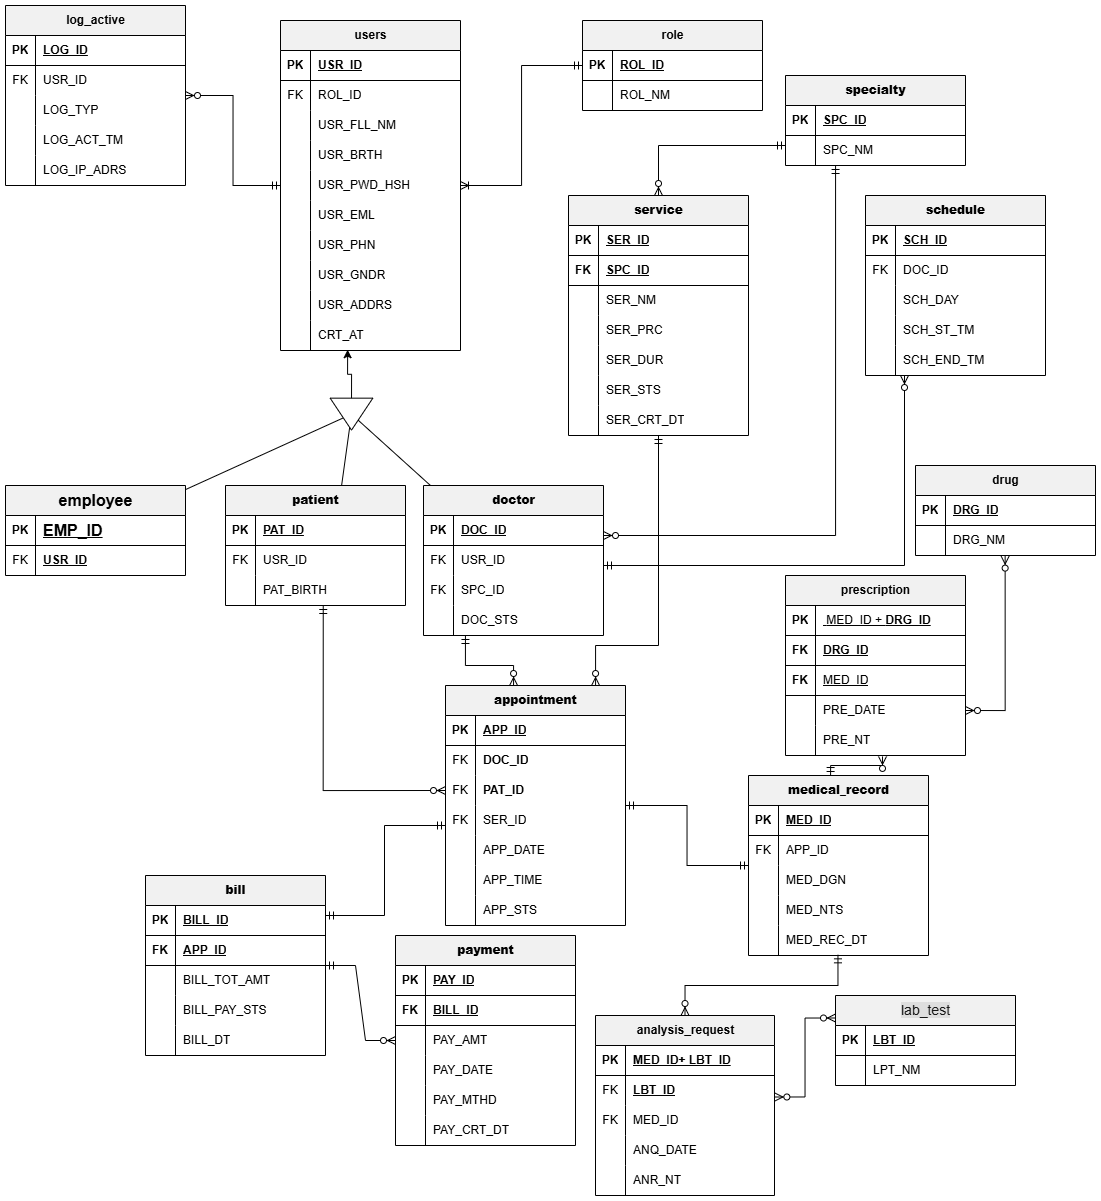
\includegraphics[width=\textwidth]{diagrams/erd.png}
	\captionof{figure}{ERD Clinic Management System }
	\label{fig:ERD}
\end{center}

The Entity-Relationship Diagram (ERD) reflects a highly normalized architecture designed to eliminate data redundancy and ensure referential integrity. The system's logic is governed by the following structural rules:
\subsubsection{Identity and Access Governance}
\begin{itemize}
	\item \textbf{Roles \& Users (1:N):} Each user is assigned a single specific role to define their access level, while a single role can be shared by multiple users.
	\item \textbf{Users \& Activity Logs (1:N):} For accountability, every system action is linked to a unique User ID, allowing the system to track multiple activities per user while maintaining a strict audit trail.
\end{itemize}
\subsubsection{Medical Infrastructure}
\begin{itemize}
	\item \textbf{Specialties, Doctors \& Services (1:N):} The \textit{Specialty} entity acts as a central hub; each specialty contains multiple doctors and services. This mandatory association ensures that patients are always directed to the correct clinical department.
	\item \textbf{Doctors \& Schedules (1:N):} A doctor can have multiple working shifts throughout the week, but each schedule entry is strictly dedicated to one specific doctor.
\end{itemize}

\subsubsection{Clinical Workflow}
\begin{itemize}
	\item \textbf{Patients \& Appointments (1:N):} A patient may book multiple appointments over time, ensuring a continuous medical history, while each appointment is tied to exactly one patient.
	\item \textbf{Appointments \& Medical Records (1:1):} To maintain clinical precision, each completed appointment generates exactly one medical record. This ensures a one-to-one correspondence between a visit and its diagnostic outcome.
	\item \textbf{Appointments \& Services (M:N):} This relationship allows an appointment to include one or more medical services, while each service can be provided across various appointments.
\end{itemize}

\subsubsection{Financial Management}
\begin{itemize}
	\item \textbf{Appointments \& Bills (1:1):} Each appointment automatically triggers the generation of a unique invoice, reflecting the costs of the rendered services.
	\item \textbf{Bills \& Payments (1:N):} The system supports multiple payment transactions for a single bill, enabling flexible payment tracking (partial or full settlements).
\end{itemize}
% ══════════════════════════════════════════════════════════════════════════════
% 0.4
% ══════════════════════════════════════════════════════════════════════════════
\subsection{Class Diagram}
\begin{center}
	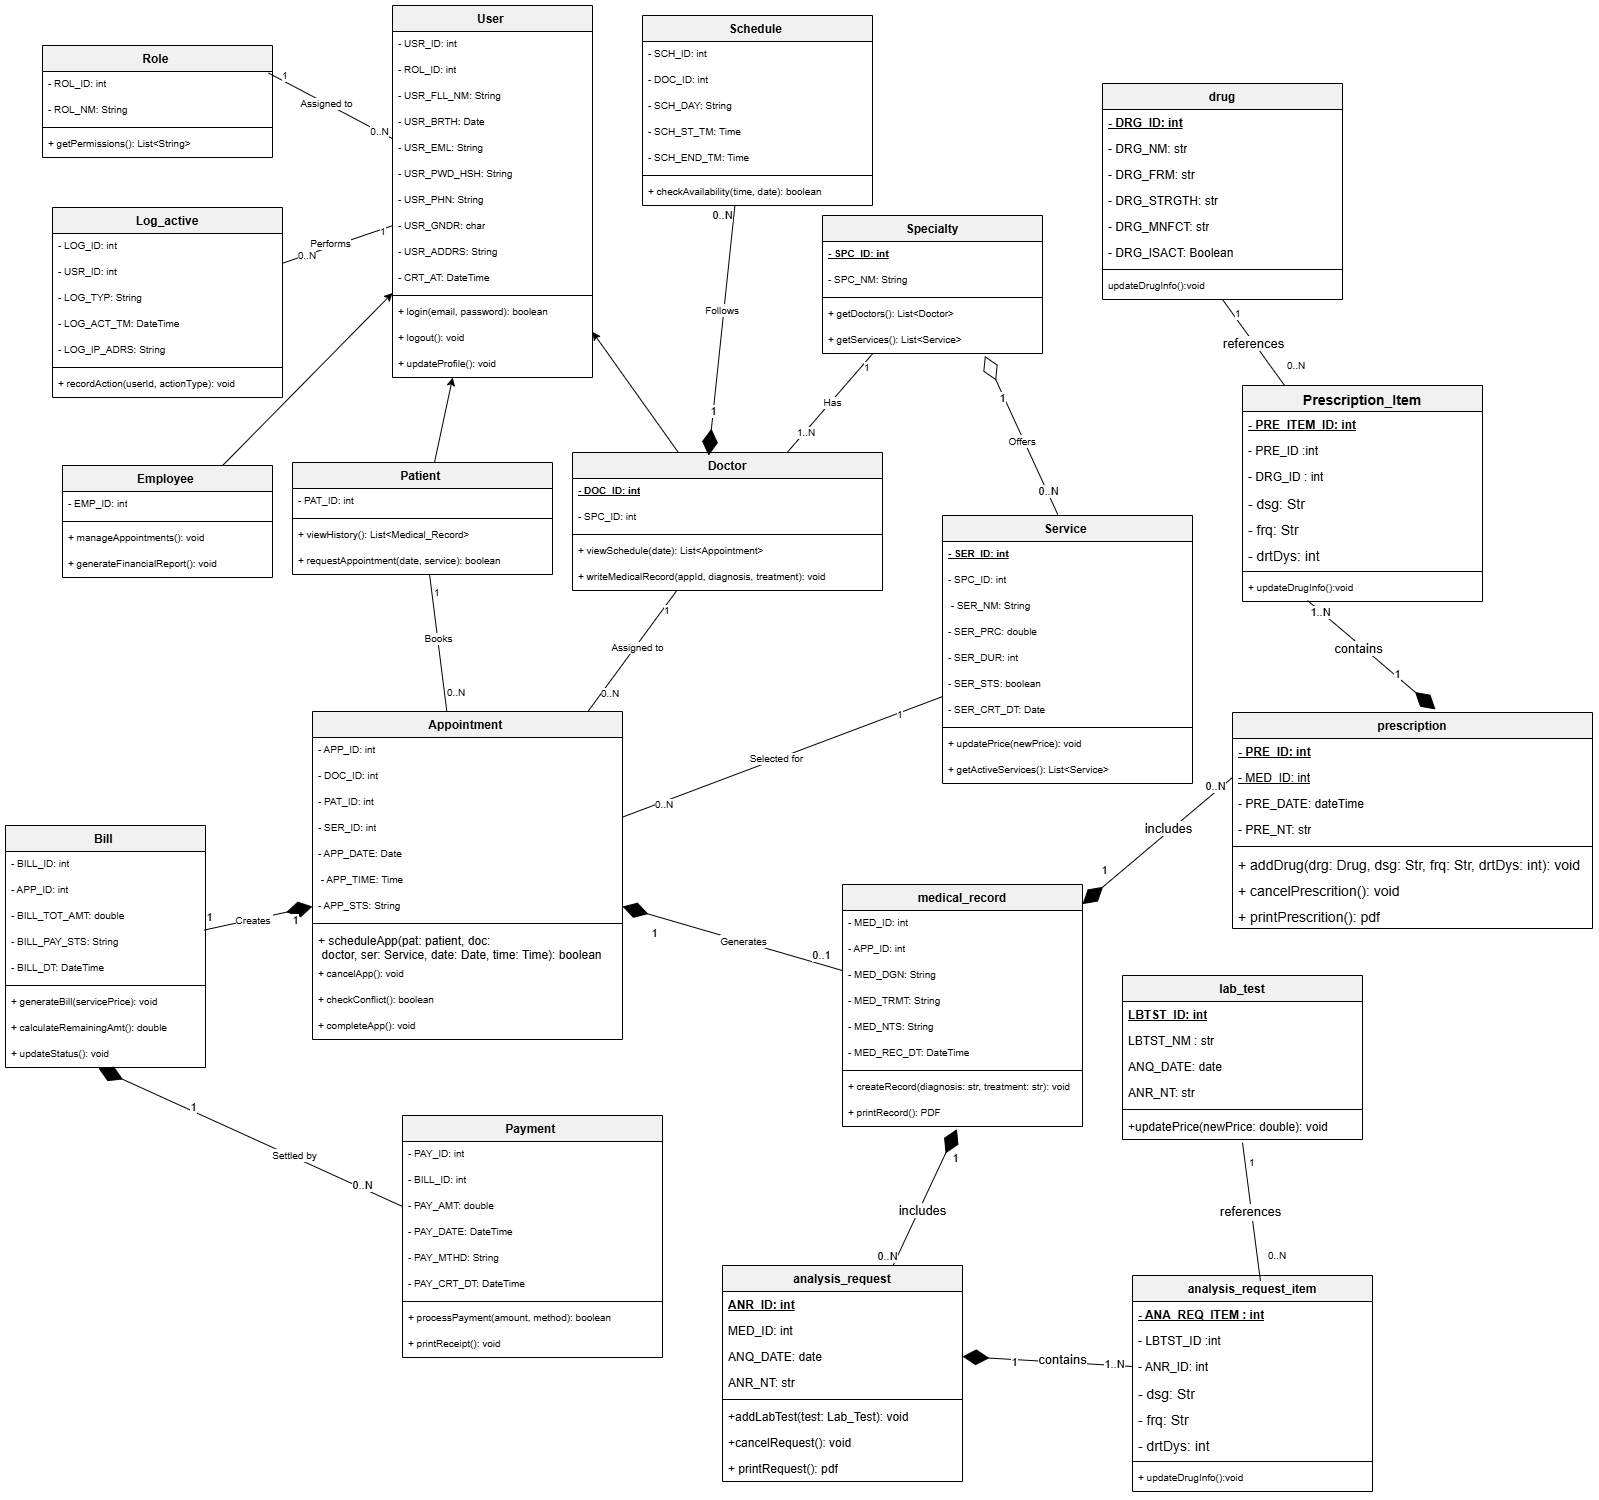
\includegraphics[width=\textwidth]{diagrams/class-diagram.png}
	\captionof{figure}{class-diagram Clinic Management System }
	\label{fig:class-diagram}
\end{center}
This Class Diagram represents the logical design of the Clinic Management System and reflects the core entities and their relationships in alignment with the SRS requirements and use case scenarios.

The diagram illustrates the complete structure of classes responsible for managing users, patients, doctors, appointments, medical records, prescriptions, laboratory analysis requests, billing, and payments. It defines the relationships using \textit{Association}, \textit{Composition}, and \textit{Aggregation} to accurately model the real operational workflow of the clinic.

The design is centered around the following key classes:
\begin{itemize}
	\item \textbf{User, Role, Log\_active}: Manage system users, permissions, and audit trail of all operations.
	\item \textbf{Patient, Doctor, Schedule, Appointment}: Handle appointment scheduling, conflict prevention, and doctor availability.
	\item \textbf{Medical\_Record, Prescription, Prescription\_Item, Drug}: Manage diagnoses, clinical notes, and electronic prescriptions linked to patient visits.
	\item \textbf{Analysis\_Request, Analysis\_Request\_Item, Lab\_Test}: Manage laboratory test requests associated with medical records.
	\item \textbf{Service, Specialty}: Organize medical services and their relation to specialties.
	\item \textbf{Bill, Payment}: Handle invoice generation, payment processing, and receipt issuance.
\end{itemize}

The diagram highlights that:

\begin{itemize}
	\item The \textbf{Appointment} class is the central entity from which both the medical record and the invoice are generated.
	\item The \textbf{Medical\_Record} contains prescriptions and laboratory analysis requests.
	\item The \textbf{Bill} is generated from the selected services during the appointment and is linked to payment transactions.
	\item All system operations are recorded in \textbf{Log\_active} to ensure full traceability and auditing.
\end{itemize}

This diagram translates the functional rules of the system into a clear object-oriented design. It serves as the foundation for both the application logic and the database schema, ensuring:

\begin{itemize}
	\item Prevention of data duplication and scheduling conflicts
	\item Strong consistency and integrity between medical and administrative entities
	\item Full support for the workflow from patient registration to payment and reporting
\end{itemize}
\subsection{Behavioral Responsibilities of Core Classes}

\begin{table}[H]
	\centering
	\small
	\renewcommand{\arraystretch}{1.4}
	\begin{tabularx}{\textwidth}{l l X}
		\toprule
		\rowcolor[gray]{0.9} \textbf{Class Name} & \textbf{Method Name} & \textbf{Functional Description} \\
		\midrule
		
		User & login() & Verifies the identity of the user (Doctor, Employee, or Patient) and grants access based on email and encrypted password. \\
		User & updateProfile() & Allows the user to update personal information such as phone number or address without administrative intervention. \\
		
		Patient & viewHistory() & Enables the patient to view all medical records and previous appointments electronically. \\
		
		Doctor & viewSchedule() & Allows the doctor to view an up-to-date list of daily appointments for better time management. \\
		Doctor & writeMedicalRecord() & Enables the doctor to record diagnosis and treatment directly into the system after consultation. \\
		
		Employee & manageAppointments() & Provides tools to create, update, or cancel appointments based on patient requests. \\
		Employee & generateFinancialReport() & Aggregates financial data to produce accurate daily or monthly income reports. \\
		
		Schedule & checkAvailability() & Checks the doctor's availability before confirming a booking to prevent overlapping appointments. \\
		
		Appointment & scheduleApp() & Creates an official booking and links it to the doctor, patient, and selected service. \\
		Appointment & checkConflict() & Prevents double-booking at the same time slot using a conflict detection algorithm. \\
		Appointment & completeApp() & Marks the appointment as completed and triggers medical record and invoice generation. \\
		
		Bill & generateBill() & Creates an invoice based on the service price associated with the appointment. \\
		Bill & calculateRemainingAmt() & Calculates the remaining amount owed in case of partial payment. \\
		
		Payment & processPayment() & Records a payment transaction including date and reference information. \\
		Payment & printReceipt() & Generates an electronic receipt confirming the paid amount. \\
		
		medical\_record & createRecord() & Archives diagnosis and treatment plan securely in the database. \\
		medical\_record & printRecord() & Allows printing an official medical report when required. \\
		
		Log\_active & recordAction() & Logs every action performed by users to maintain a complete audit trail. \\
		
		\bottomrule
	\end{tabularx}
\end{table}